\documentclass[12pt]{article}
\usepackage{../../../lecture_notes}
\usepackage{../../../math}
\usepackage{../../../uark_colors}

\hypersetup{
  colorlinks = true,
  allcolors = ozark_mountains,
  breaklinks = true,
  bookmarksopen = true
}

\begin{document}
\begin{center}
  {\Huge\bf Final - Fall 2025}
  
  \smallskip
  {\large\it ECON 4753 — University of Arkansas}
\end{center}

\vspace{5mm}
The following question is based on data collected about faculty at UT Austin and each instructor's average course evaluations. 
There are a total of 463 instructors with 195 being female and 268 being male.
For male instructors the average rating is $\bar{y}_M = 4.07$ and a standard deviation of $\sigma_{y, M} = 0.56$.
For female instructors the average rating is  $\bar{y}_F = 3.90$ and a standard deviation of $\sigma_{y, M} = 0.54$.

Regressing evaluations on an indicator for being a male instructor produces the following output:

  \begin{smallcodeblock}[{}]
OLS estimation, Dep. Var.: eval
Observations: 463
Standard-errors: IID 
             Estimate Std. Error  t value  Pr(>|t|)    
(Intercept)  3.901026   0.039330 99.18747 < 2.2e-16 ***
gender::male 0.168004   0.051695  3.24994 0.0012388 ** 
---
Signif. codes:  0 '***' 0.001 '**' 0.01 '*' 0.05 '.' 0.1 ' ' 1
  \end{smallcodeblock}

\begin{enumerate}
  \item What is the sample distribution of the male-specific sample mean of the evaluation?
  
  \item Form a 90\% confidence interval around the male specific sample mean (the critical value is $1.65$). Interpret this confidence interval in words.
  
  \item Do male and female instructors have different average ratings? Is this difference statistically significant?
\end{enumerate}

\newpage
%% Question on Diamonds' sale price
The following questions are based on data about diamond sales prices and their characteristics. 
For each diamond, we record their cut (Fair, Good, Very Good, Premium, and Ideal) as well as their caret.
For this question, I created bins of caret size: 0--0.5, 0.5--1, 1--2, and 2+ carets.

The regression examines how diamond cut quality affects price while controlling for carat size.

  \begin{smallcodeblock}[{}]
                                 est_lin             est_bin
Dependent Var.:                    price               price
                                                            
Constant             -3,875.5*** (51.16)      121.4* (60.48)
cut = Good            1,120.3*** (55.00)    573.8*** (66.74)
cut = VeryGood        1,510.1*** (52.73)    725.1*** (62.97)
cut = Premium         1,439.1*** (53.21)    697.9*** (63.34)
cut = Ideal           1,800.9*** (51.69)    762.1*** (61.60)
carat                 7,871.1*** (24.88)                    
carat_bin = 0.5<x<=1                      2,005.0*** (10.49)
carat_bin = 1<x<=2                        6,796.1*** (26.58)
carat_bin = x>=2                         14,164.6*** (60.88)
____________________ ___________________ ___________________
  \end{smallcodeblock}


\begin{enumerate}
  \setcounter{enumi}{3}
  \item When modeling the relationship between carat size and diamond price, you could either use carat as a linear term or create bins/categories. 
  What are the advantages and disadvantages of using carat as a linear term versus creating bins (e.g., small, medium, large diamonds)?
  
  \bigskip
  \item Consider the regression in the first column (with the linear term for `carat'). 
  Interpret the coefficient on \texttt{Premium} in words. Comment on it's statistical significance.
  
  \bigskip
  \item Consider the regression in the first column (with the linear term for `carat'). The regression controls for carat size when examining the relationship between cut and sales price.
  \begin{enumerate}[label=(\alph*)]
    \item Why is it important to control for carat size when trying to understand the effect of cut quality on diamond prices?
    
    \item Interpret the coefficient on carat in words. Include a 95\% confidence interval for this coefficient when interpreting.
  \end{enumerate}
\end{enumerate}




\newpage
The following questions are based on monthly data on US natural gas consumption in and the average temperature (Fahrenheit) in NYC's central park. 
See the figure and regression table on the next page.

\begin{enumerate}
  \setcounter{enumi}{6}
  \item The time-series data clearly shows seasonal patterns with higher consumption in the winter months. Which term(s) in my time-series regression estimate these patterns?
  
  \bigskip
  \item The regression includes a continuous \texttt{date} variable to capture the time trend. 
  Interpret the coefficient on \texttt{date} in words. 
  What does it tell us about natural gas consumption over time?
  
  \bigskip
  \item Interpret the coefficient on \texttt{avg\_temp} in words. 
  
  \bigskip
  \item If we remove the \texttt{avg\_temp} term in the regression, the month with the highest natural gas consumption is January. 
  Why do you think controlling for average temperature changed this? 
\end{enumerate}



\newpage
\begin{figure}[!th]
  \caption{Natural Gas Consumption and NYC Average Temperature}
  \label{fig:f1}
  
  \vspace*{-2\bigskipamount}
  \begin{center}
    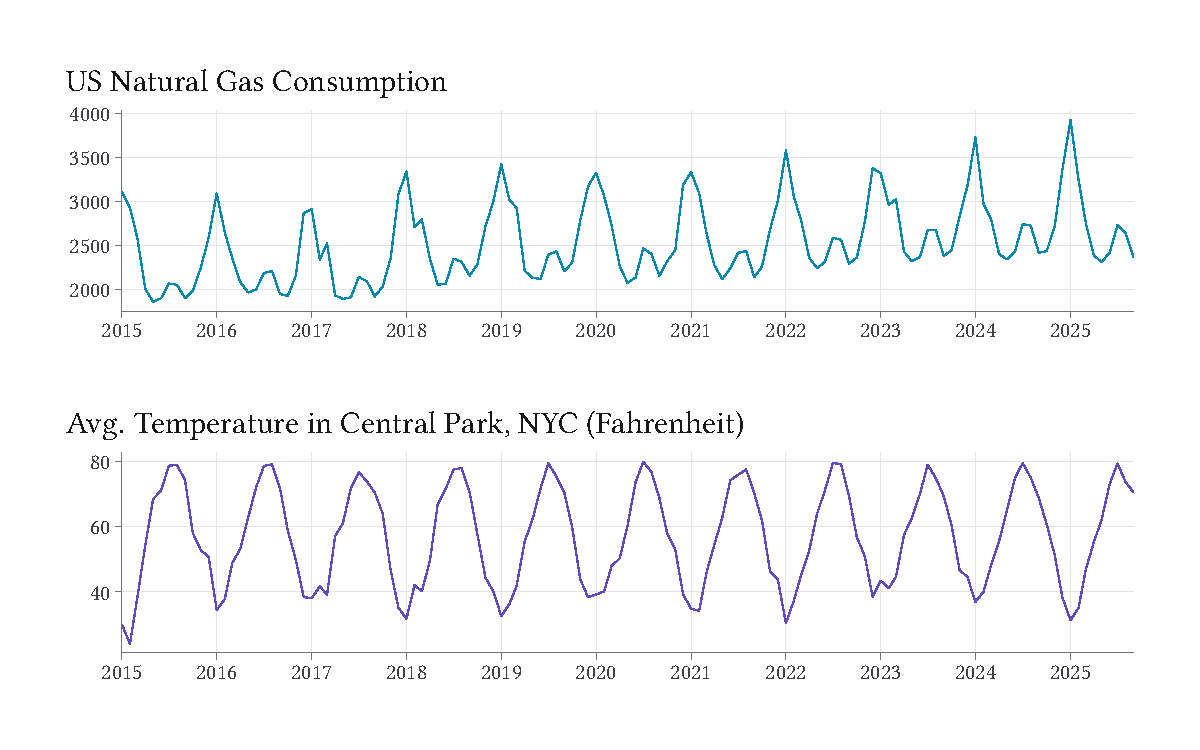
\includegraphics[width = 0.9\textwidth]{figures/p_natural_gas_and_temp.pdf}
  \end{center}
\end{figure}

  \begin{smallcodeblock}[{}]
OLS estimation, Dep. Var.: natural_gas
Observations: 129
Standard-errors: Heteroskedasticity-robust
                               Estimate Std. Error t value   Pr(>|t|)
(Intercept)                     1245.00    1.5e+02    8.33 1.9168e-13 ***
date                               0.16    7.6e-03   21.05  < 2.2e-16 ***
month(date, label = TRUE)::Feb  -410.92    5.2e+01   -7.93 1.5862e-12 ***
month(date, label = TRUE)::Mar  -448.72    6.0e+01   -7.45 1.9206e-11 ***
month(date, label = TRUE)::Apr  -705.47    7.1e+01   -9.98  < 2.2e-16 ***
month(date, label = TRUE)::May  -624.59    9.2e+01   -6.79 5.0866e-10 ***
month(date, label = TRUE)::Jun  -374.43    1.1e+02   -3.32 1.2172e-03 **
month(date, label = TRUE)::Jul    22.44    1.3e+02    0.17 8.6704e-01
month(date, label = TRUE)::Aug   -46.41    1.3e+02   -0.36 7.2256e-01
month(date, label = TRUE)::Sep  -434.92    1.1e+02   -4.01 1.0648e-04 ***
month(date, label = TRUE)::Oct  -589.90    8.4e+01   -7.04 1.4664e-10 ***
month(date, label = TRUE)::Nov  -511.13    6.5e+01   -7.85 2.4482e-12 ***
month(date, label = TRUE)::Dec  -181.61    4.4e+01   -4.11 7.5305e-05 ***
avg_temp                         -22.64    2.8e+00   -8.11 6.2811e-13 ***
  \end{smallcodeblock}



\end{document}
